\documentclass[xcolor={dvipsnames}]{beamer}

\usetheme{Malmoe}
\usecolortheme{seagull}
\usepackage[]{natbib}
\usepackage{textpos}
\usepackage{amsmath, amssymb, bm}
\usepackage{multirow}
\usepackage{framed}
\usepackage{schemata}
\setbeamertemplate{navigation symbols}{}
\usepackage[english]{babel}
\usepackage{animate}
\usepackage{graphics}
\usepackage{fontawesome}
\usepackage{tikz,graphicx}

\definecolor{lightblue}{rgb}{0.145,0.6666,1} % Defines the color used for content box headers
\definecolor{Red}{rgb}{0.9,0.15,0}
\definecolor{Blue}{RGB}{55,126,184}
\definecolor{Green}{RGB}{77,175,74}
\definecolor{White}{RGB}{255,255,255}
\definecolor{Lightgray}{rgb}{0.86,0.86,0.86}

\setbeamertemplate{footline}
{
	\leavevmode%
	\hbox{%
		\begin{beamercolorbox}[wd=.50\paperwidth,ht=2.25ex,dp=1ex,center]{author in head/foot}%
			\usebeamerfont{author in head/foot}\insertshortauthor%% \beamer@ifempty{\insertshortinstitute}{}{(\insertshortinstitute)}
		\end{beamercolorbox}%
%		\hskip2pt%
		\begin{beamercolorbox}[wd=.50\paperwidth,ht=2.25ex,dp=1ex,center]{title in head/foot}%
			\usebeamerfont{title in head/foot}\insertshorttitle~~~~~~~~~~~~~~~~~~~~~~~~~~\insertframenumber
		\end{beamercolorbox}%
	}%
	\vskip0pt%
}
\makeatother

\title[COVID-19 and life expectancy]{}

%\subtitle{\large{\textsc{ Leveraging demographic science to uncover trends of violence during the COVID-19 pandemic in the UK, Italy, and Mexico}}\\$\,$\\}


\author[LCDS meeting February 15 2020]
{
	\vspace{-0.5cm}
	\texorpdfstring{
		\begin{columns}
			\column{1\linewidth}
			\centering
			\Large{\textbf{Recent Gains in Life Expectancy Reversed by the Covid-19 Pandemic}\\}
			$\,$\\
			LCDS meeting February 15 2021\\
			\begin{center}						
			
\includegraphics[scale=0.4]{logos_sdu_lcds.png}\\
			\end{center} 
				$\,$\\    
				\vspace{0.5cm}
						%\includegraphics[scale=0.2]{Figs/MPIDR.PNG}   
		\end{columns}
	}
	{Jos\'{e} Manuel Aburto}
}

\date[]{February 2021}

\beamertemplatenavigationsymbolsempty
\begin{document}


\begin{frame}[plain]
	\titlepage
\end{frame}
%%%%%%%%%%%%%%%%%%%%%%%%%%%%%%%%%%%%%%%%%%%%%%%%%%%%%%%%%%%%%%%%%%%%%%%%%
%%%%%%%%%%%%%%%%%%%%%%%%%%%%%%%%%%%%%%%%%%%%%%%%%%%%%%%%%%%%%%%%%%%%%%%%%


%%%%%%%%%%%%%%%%%%%%%%%%%%%%%%%%%%%%%%%%%%%%%%%%%%%%%%%%%%%%%%%%%%%%%%%%%


\begin{frame}
\Large{
	\begin{center}
		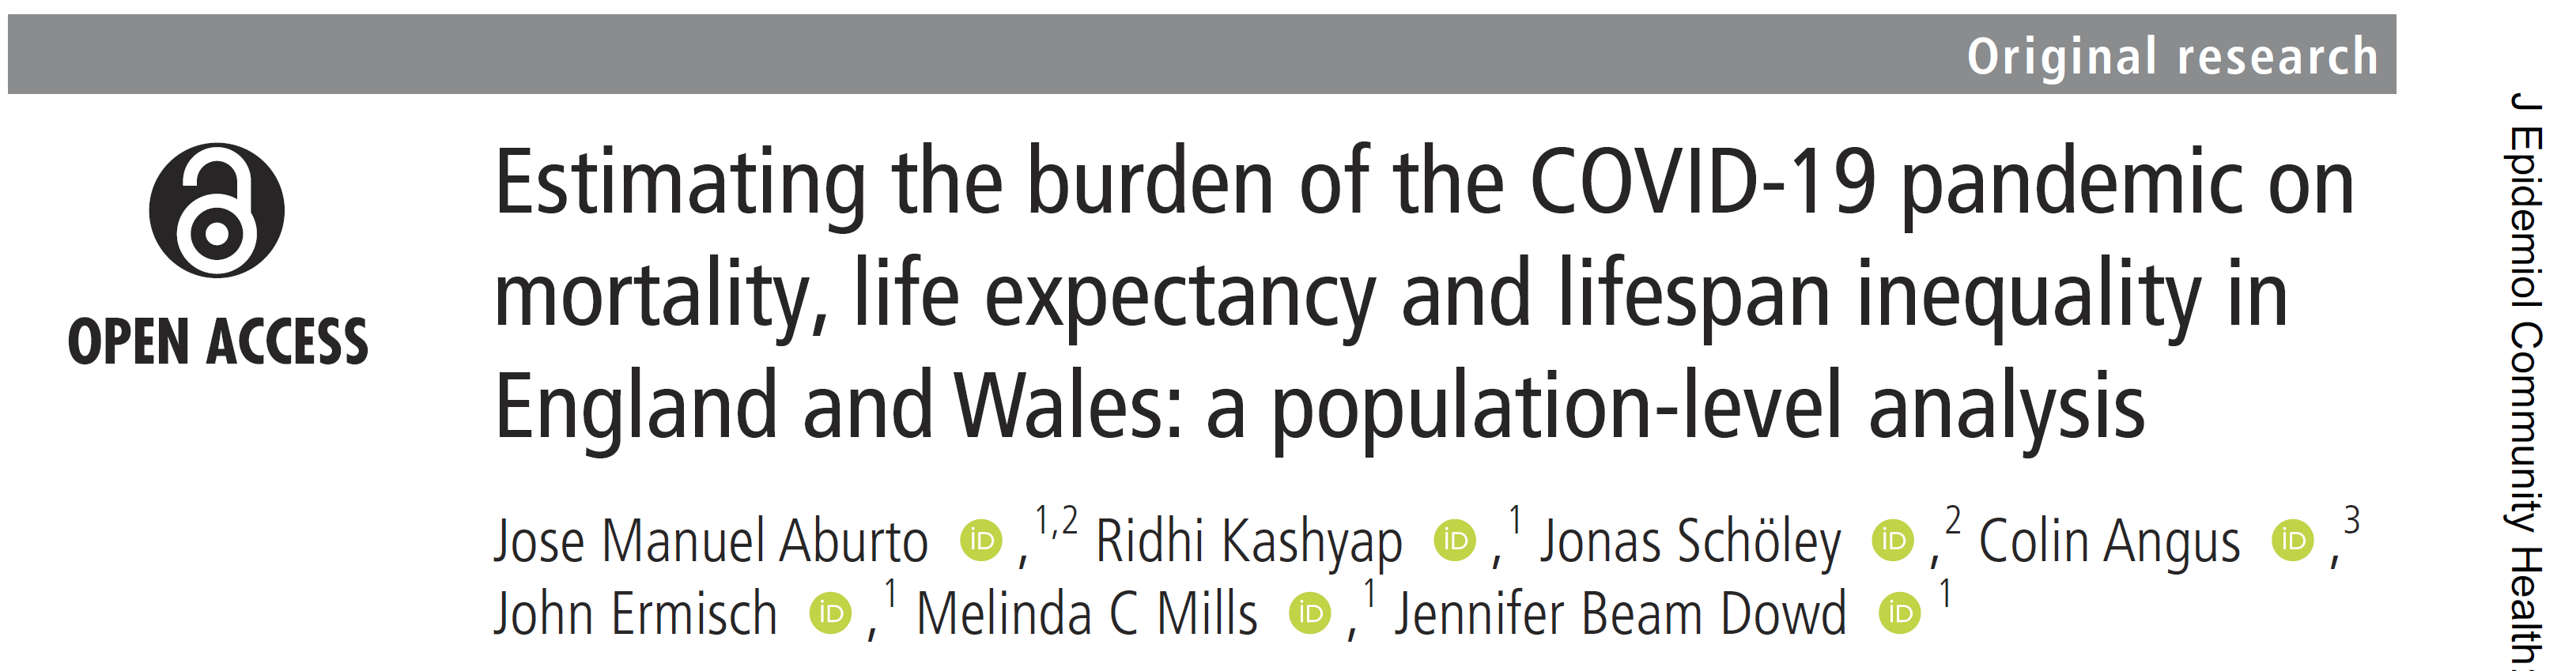
\includegraphics[scale=.3]{Fig_jech}
	$\,$\\

\pause

\textbf{To document the cumulative burden of the pandemic on life expectancy in a cross-national, comparative perspective.}

\end{center} 

}
\end{frame}

\begin{frame}
\Large{
	\begin{center}
		\textbf{Life expectancy at birth ($e_0$)} \linebreak
		
		Average number of years a cohort of newborns would live if they were to experience the death rates  in a given year.
\end{center} 

\pause
\begin{itemize}
\item Widely-used metric of pop health and \textbf{longevity}.

\item \textbf{Unaffected} by population structure.

\item Enables \textbf{comparisons}.

\item Can be \textbf{decomposed} by age and CoD.

\end{itemize}

}
\end{frame}


\begin{frame}
\Large{
	\begin{center}
		\textbf{Life expectancy levels}
		
			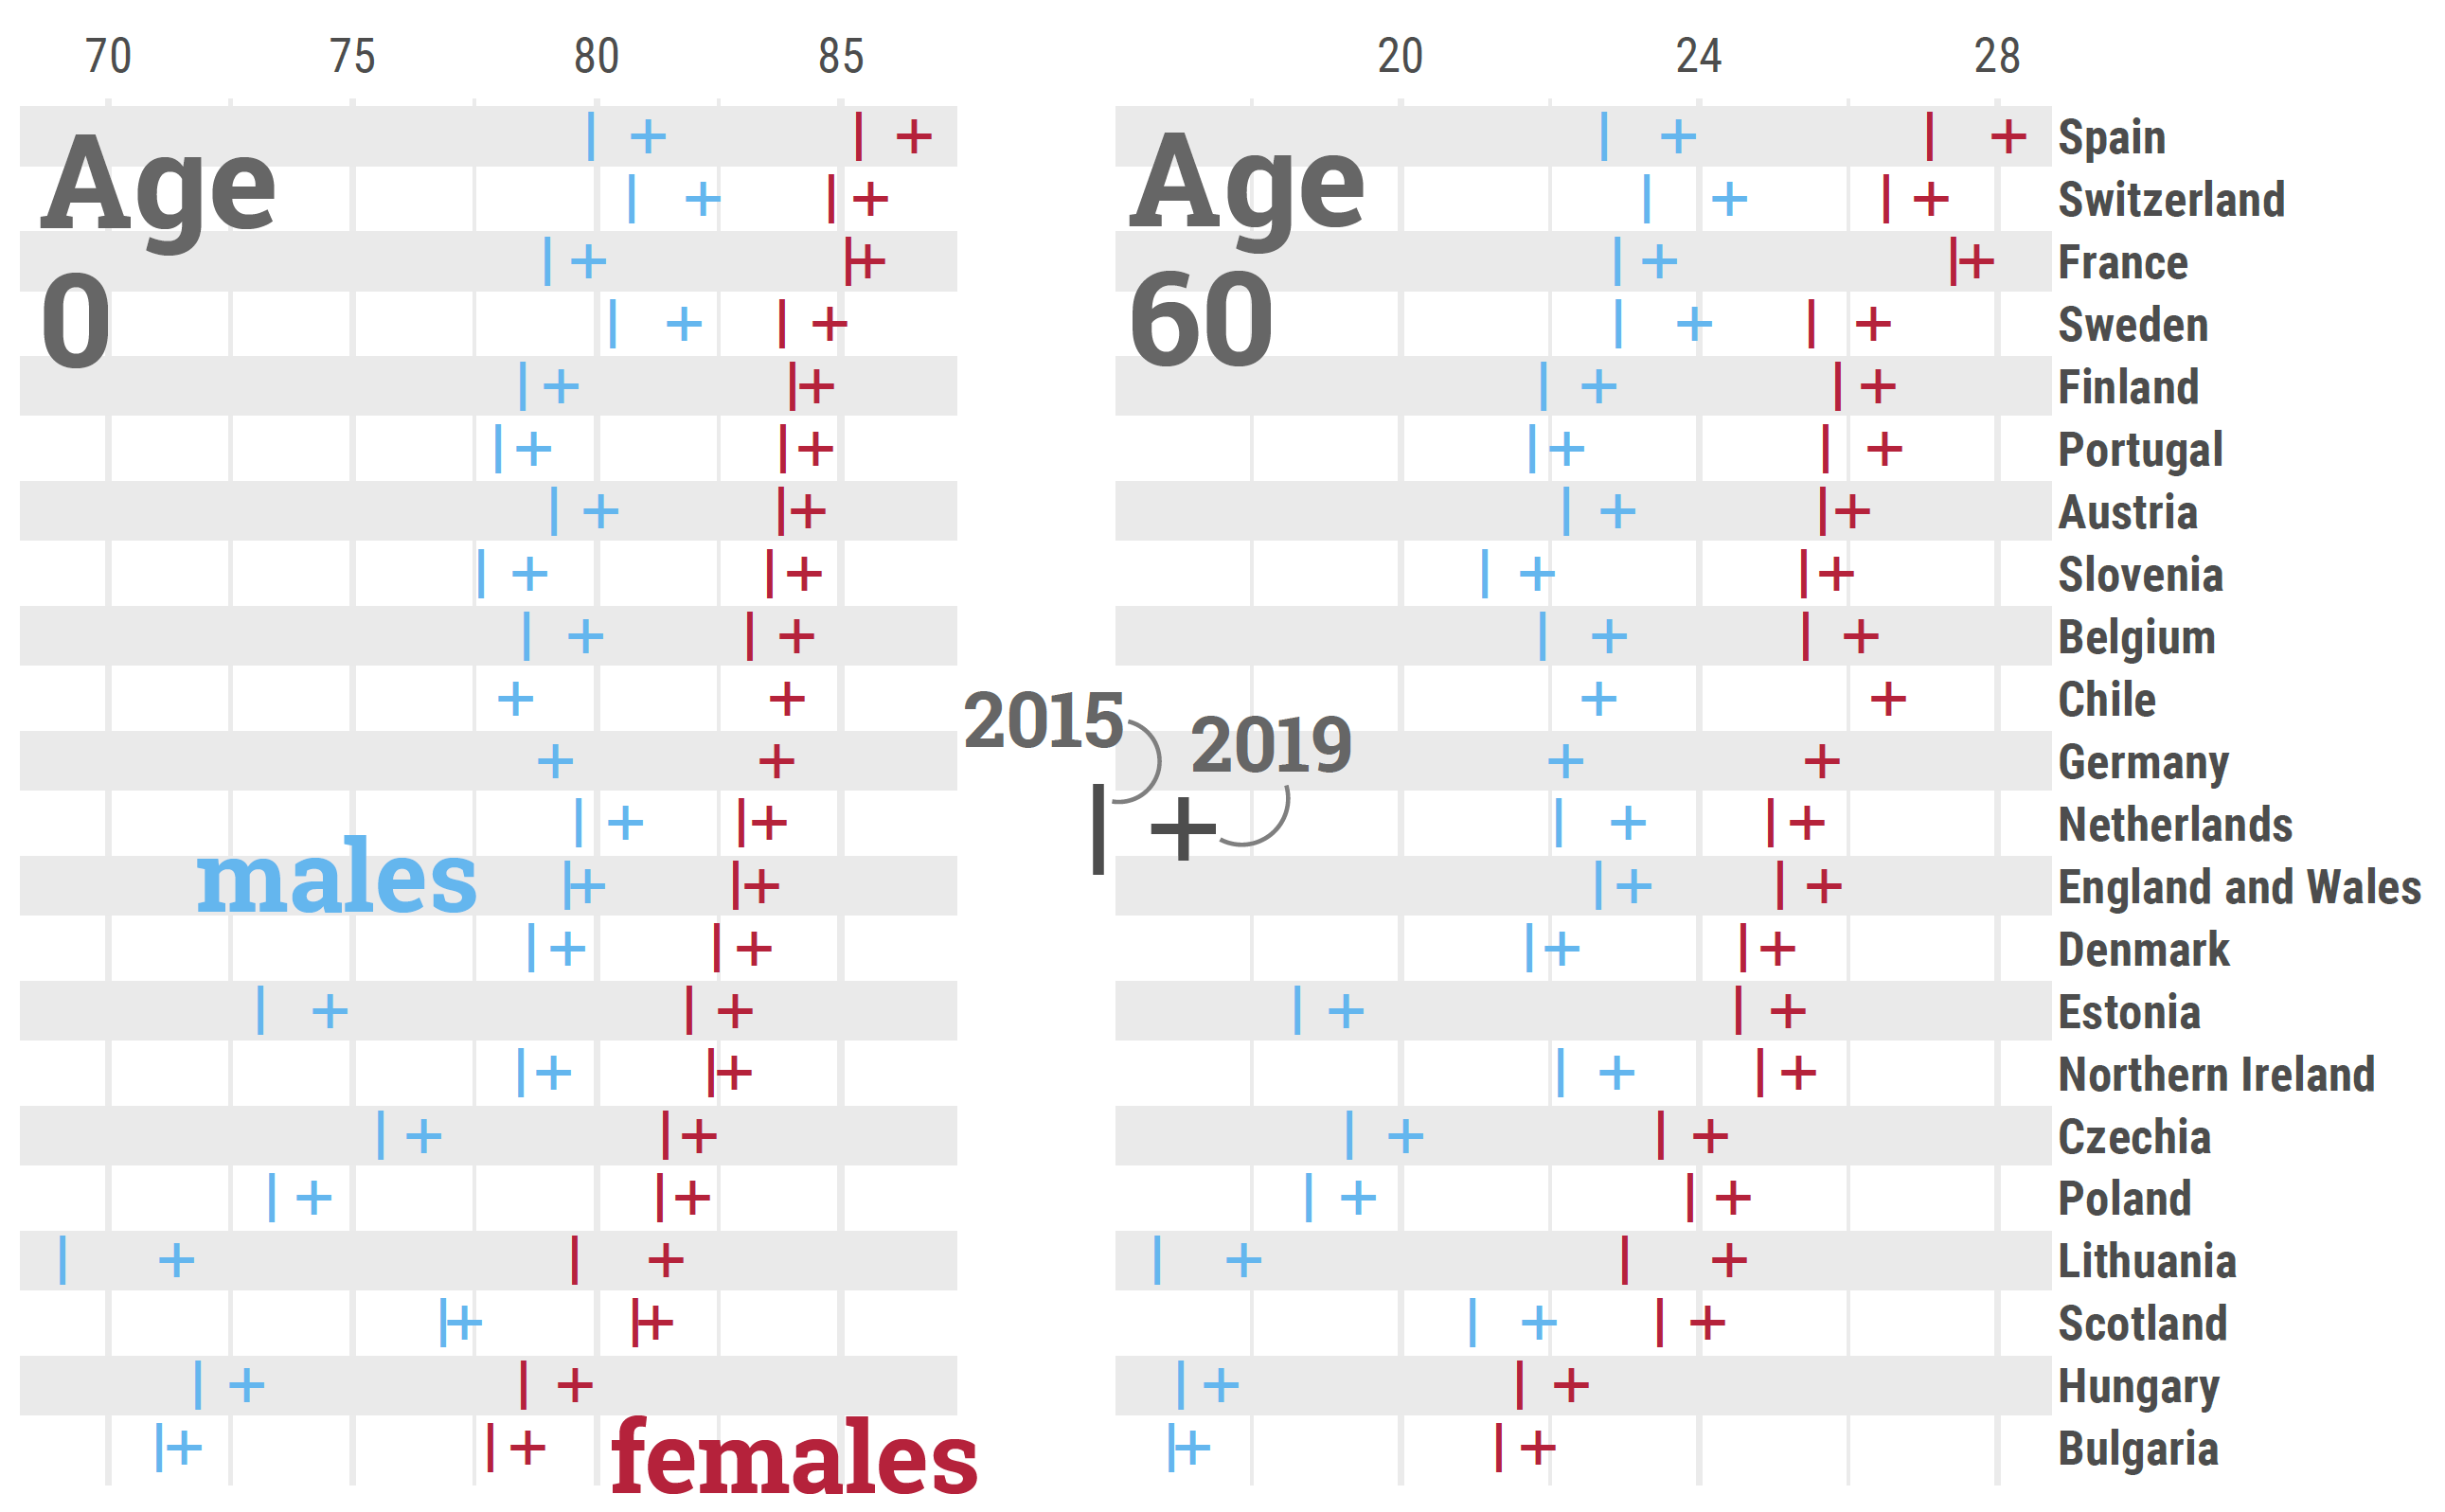
\includegraphics[scale=.38]{Fig_levels}
	\end{center} 
}
\end{frame}

\begin{frame}
\Large{
	\begin{center}
		\textbf{Contributions of this study}
	\end{center} 
	\pause
	\begin{itemize}
	\item \textbf{Harmonization} of data by age and sex for 23 countries. \pause
	\item Report life expectancy for \textbf{2019} and \textbf{2020}. \pause
	\item \textbf{Quantify} $e_0$ losses during the pandemic. \pause
	\item Disentangle the \textbf{ages} that contributed to these losses. \pause
	\item For 13 countries, linked attributable losses to \textbf{COVID-19}.
	\end{itemize}
}
\end{frame}

\begin{frame}
\Large{
	\begin{center}
		\textbf{Context before the pandemic}
	\end{center} 
	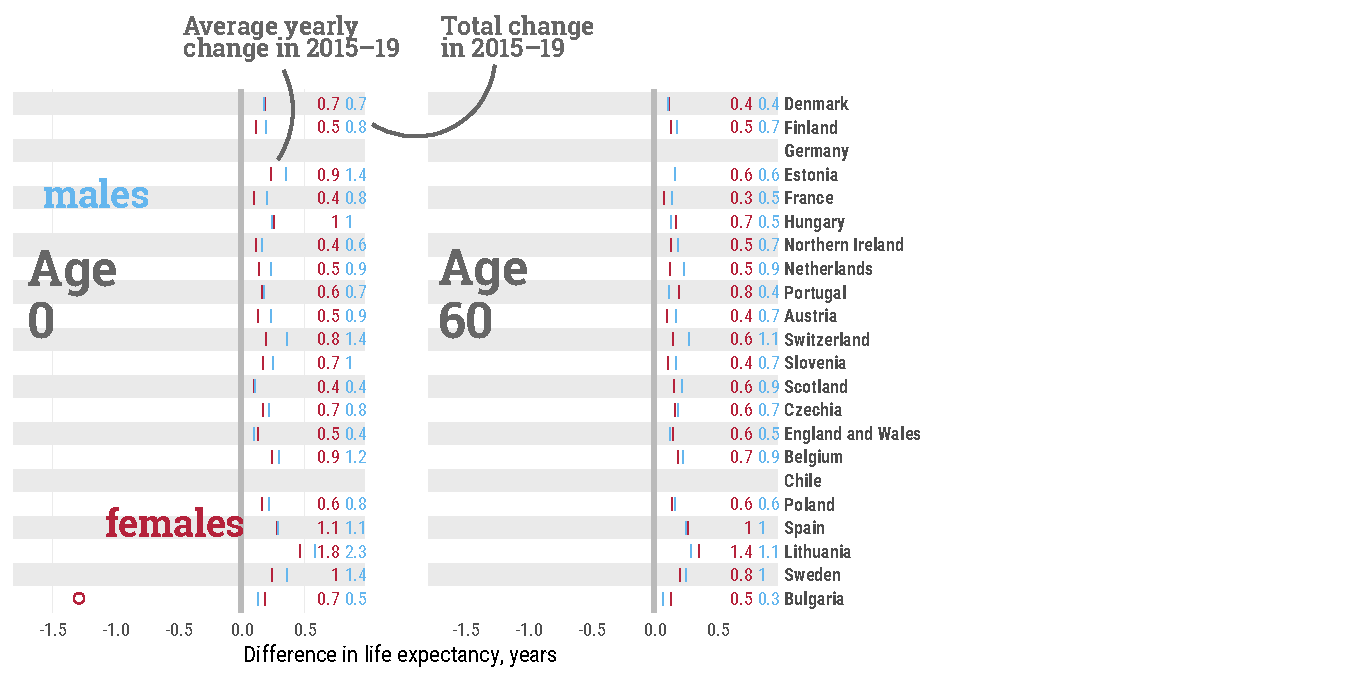
\includegraphics[scale=.72]{fig-2-ann0}	
}
\end{frame}


\begin{frame}
\Large{
	\begin{center}
		\textbf{Context during the pandemic}
	\end{center} 
	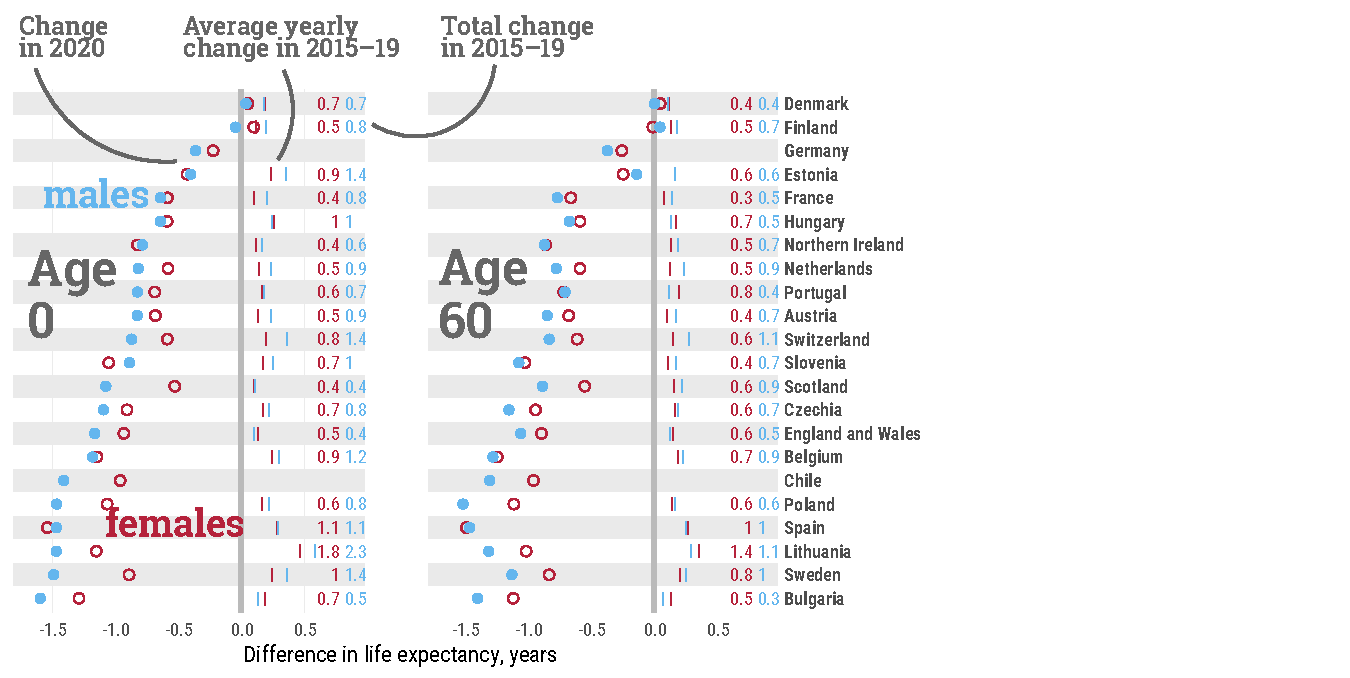
\includegraphics[scale=.72]{fig-2-ann}	
}
\end{frame}

\begin{frame}
\Large{
	\begin{center}
		\textbf{Ages driving losses}
		\hspace*{-1cm}   
		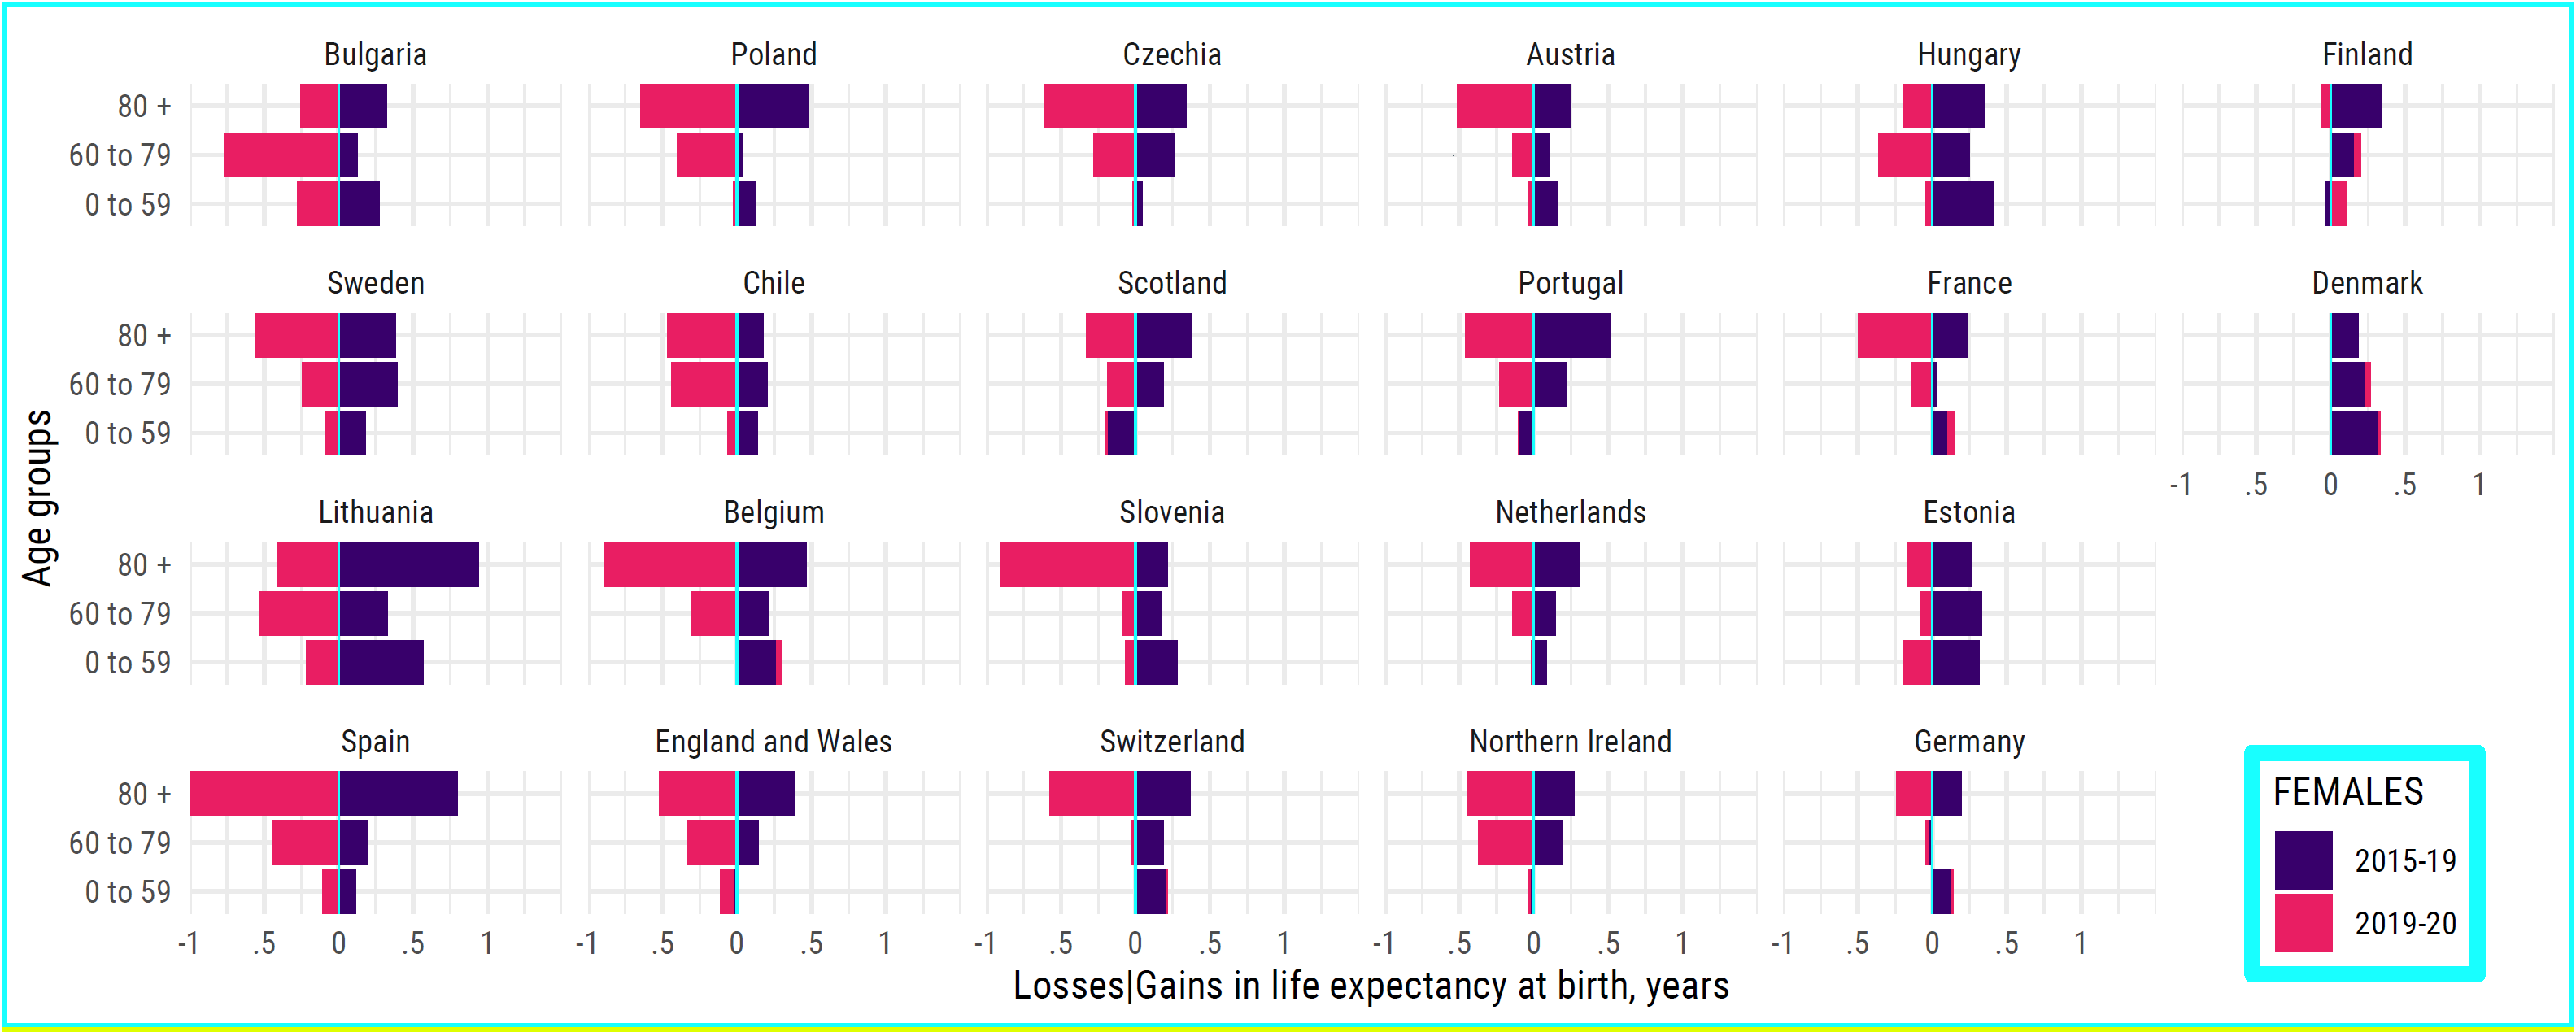
\includegraphics[scale=.34]{decomp_females}	
	\end{center} 
}
\end{frame}

\begin{frame}
\Large{
	\begin{center}
		\textbf{Ages driving losses}
		\hspace*{-1cm}   
		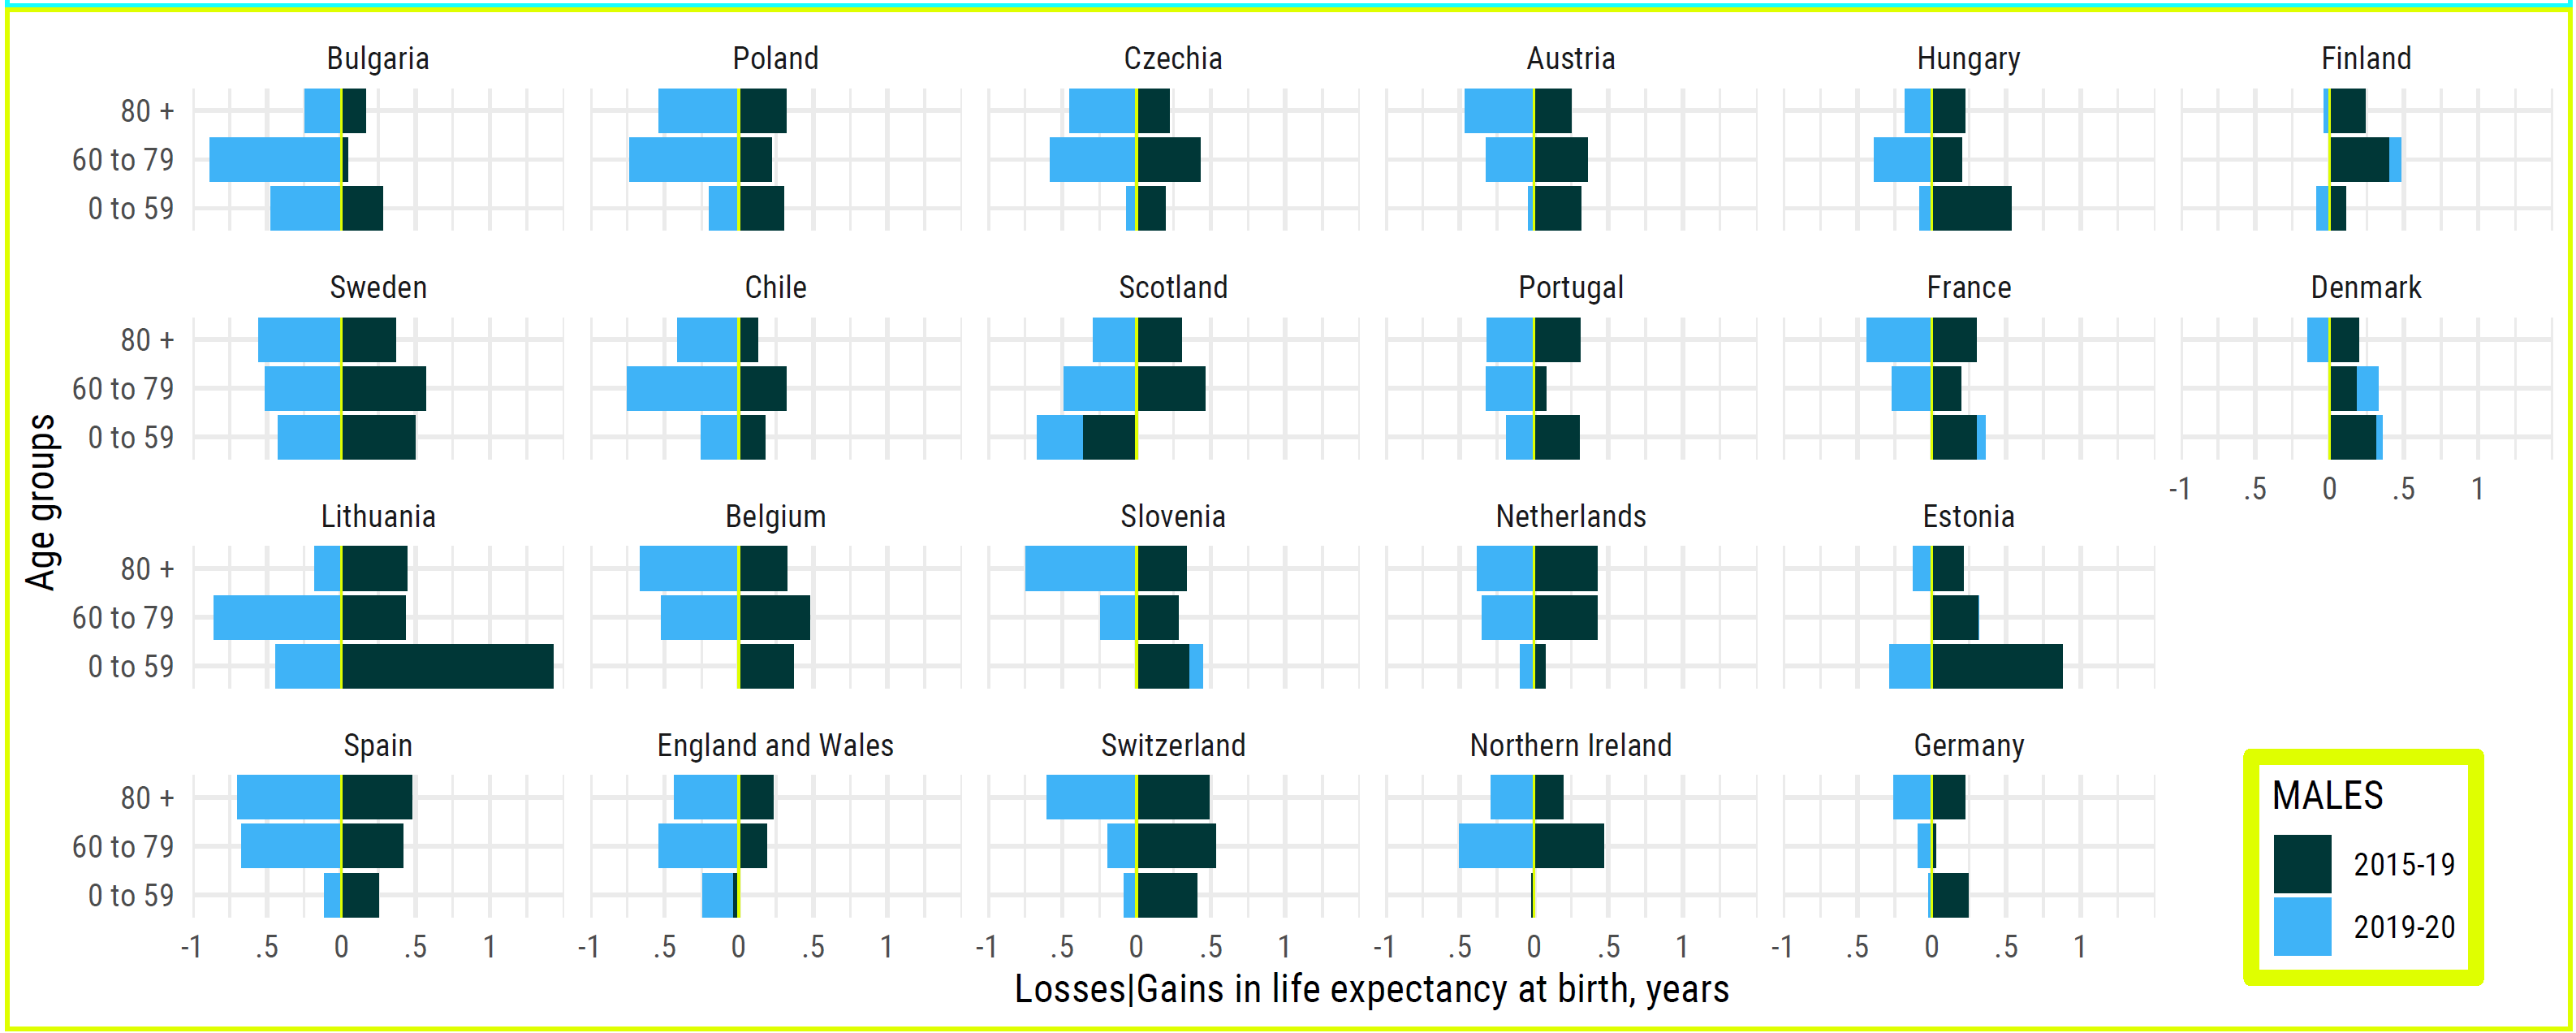
\includegraphics[scale=.34]{decomp_males}	
	\end{center} 
}
\end{frame}

\begin{frame}
\Large{
	\begin{center}
		\textbf{COVID-19 attributable losses}
	\end{center} 
		\hspace*{-1.8cm}   
	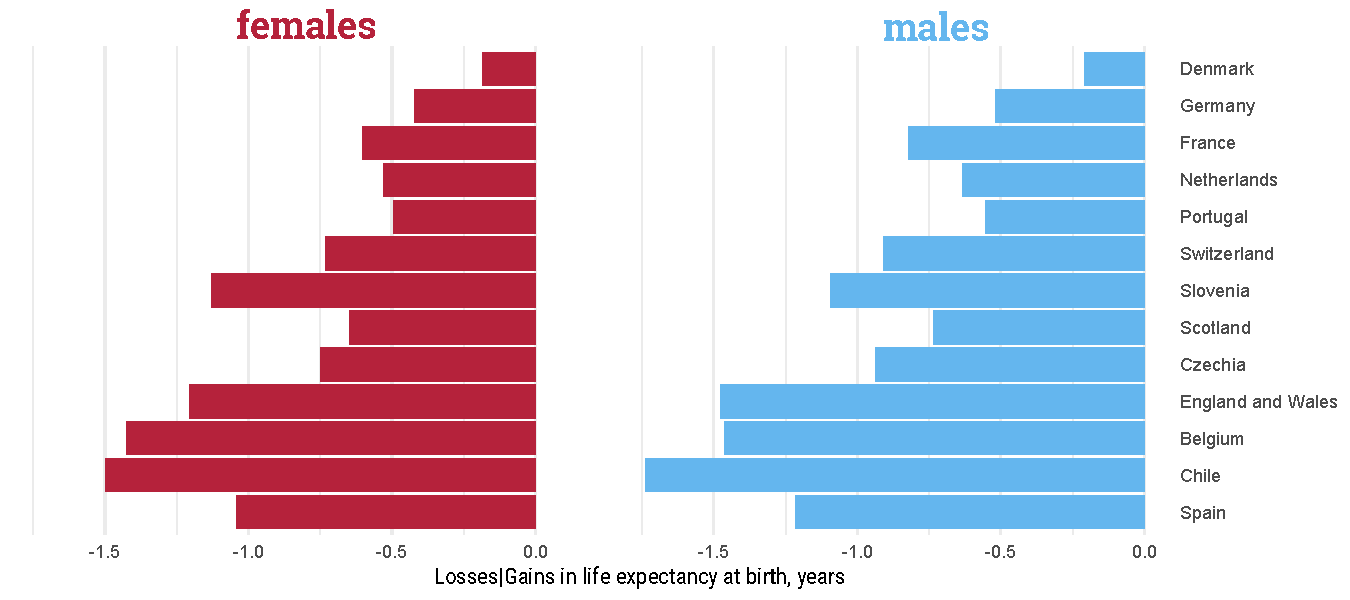
\includegraphics[scale=.58]{fig-4}
}
\end{frame}


\begin{frame}
\Large{
	\begin{center}
		\textbf{Conclusions}
	\end{center} 
\begin{itemize}
\item The COVID-19 pandemic halted longevity improvements in 2020. \pause
\item Most countries experienced substantial losses in $e_0$. \pause
\item Mostly attributed to mortality above age 60 and to COVID-19 deaths. \pause
\item More efforts are needed to report timely data. \pause
\item The recovery of life expectancy in the short-term remains uncertain. 

\end{itemize}
}
\end{frame}

	

%%%%%%%%%%%%%%%%%%%%%%%%%%%%%%%%%%%%%%%%%%%%%%%%%%%%%%%%%%%%%%%%%%%%%%%%

%%%%%%%%%%%%%%%%%%%%%%%%%%%%%%%%%%%%%%%%%%%%%%%%%%%%%%%%%%%%%%%%%%%%%%%%
\begin{frame}
\Large{
 \begin{center}
	\begin{center}
	 \textbf{Recent Gains in Life Expectancy Reversed by the Covid-19 Pandemic}\linebreak
	 
	\hspace*{2cm}   
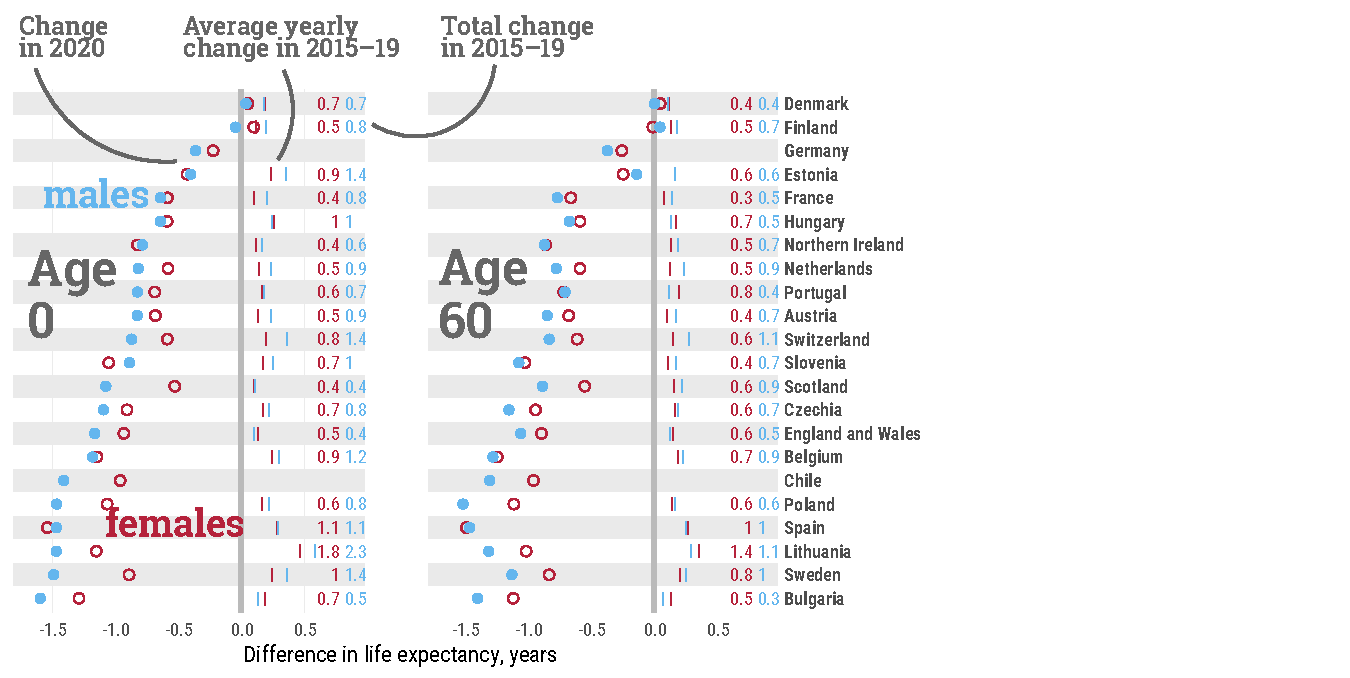
\includegraphics[scale=.3]{fig-2-ann}\linebreak
	\end{center}
 
José Manuel Aburto, Jonas Schöley, Luyin Zhang, Ilya Kashnitsky, Charles Rahal, Trifon Missov, Melinda Mills, Jenn B. Dowd, Ridhi Kashyap


\end{center}
}
\end{frame}



\end{document}
	

